\subsection{Skewed-Astroid parametric equation}

\begin{table}[ht]
	\begin{center}
		\begin{tabular}[top]{ |p{16.0 cm}| }
			\rowcolor{LIGHTCYAN}			
		%%	\hline \multicolumn{1}{|c|}{\textbf{Part 2/5 Ellipse and Skewed-Astroid parametric curves}} \\ [1.0ex]
	
			\rowcolor{LIGHTCYAN}
			\hline \textbf{No. 4 - Skewed-Astroid parametric curve}\\
			\begin{eqnarray}
				x(u) & = & 40  [ \sin(2\pi u) ]^3  \nonumber \\
				y(u) & = & 100 [ \cos(2\pi u) ]^3  \nonumber \\
				u & \in & [0.0, 1.0] \nonumber
			\end{eqnarray}
			
			
			Closed loop\\
			Overall Single loop, 4 cusps and 4 concave curves \\
			Reflection x-axis: symmetrical\\
			Reflection y-axis: symmetrical\\
			\frame{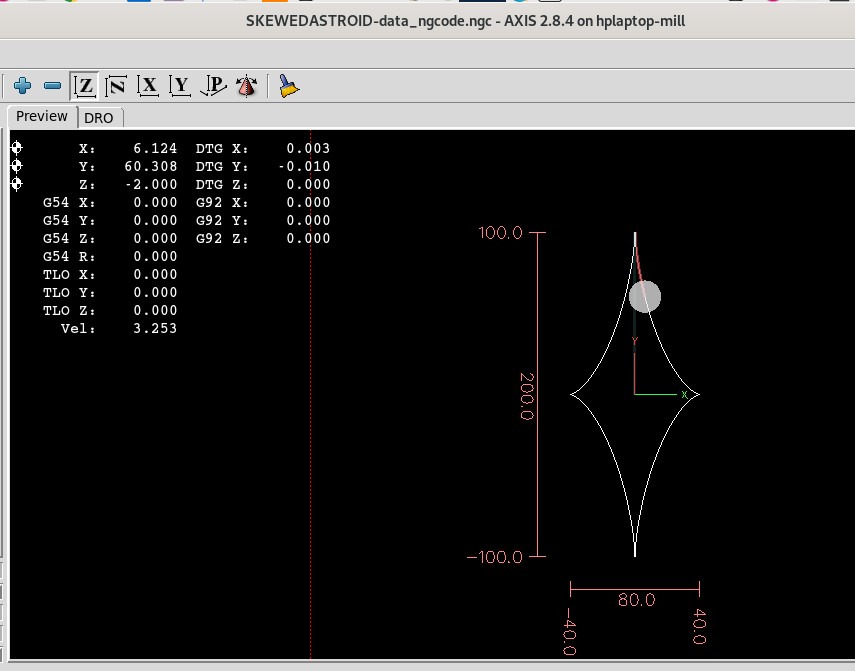
\includegraphics[width=0.51\textwidth]{./07-images/img-Ch5/SKEWED-ASTROID-Axis.png}}
			\frame{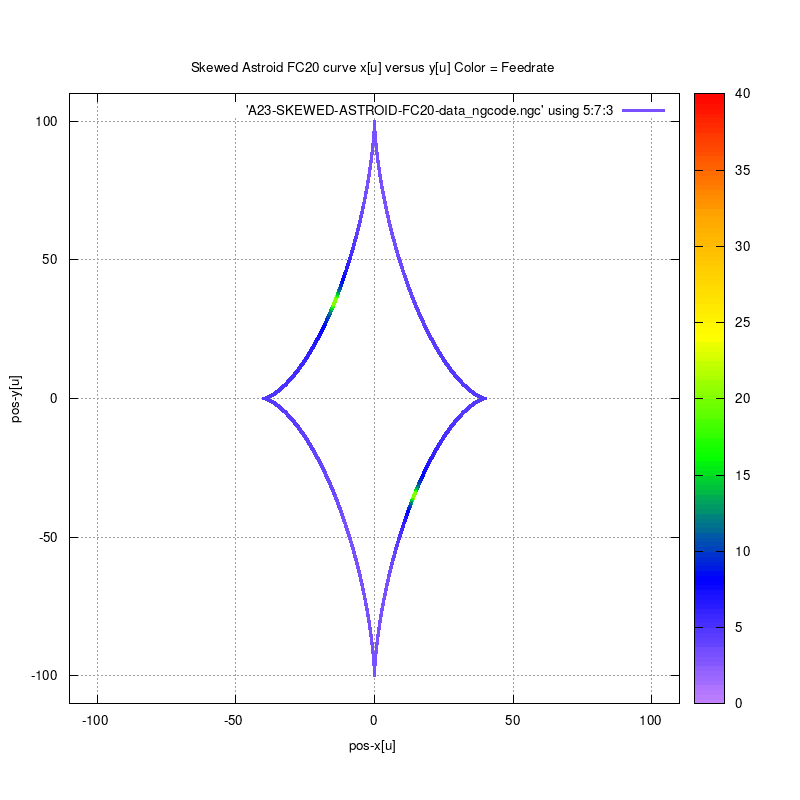
\includegraphics[width=0.40\textwidth]{./07-images/img-Ch5/SKEWED-ASTROID-Feedrate.png}}\\
			
			\hline
		\end{tabular}
		\caption{Skewed-Astroid and dimensions }		
		\label{table:Skewed-Astroid equation and dimensions}
	\end{center}
\end{table}  
